\documentclass[a4paper]{article}
\usepackage[brazil]{babel} 
%\usepackage[english]{babel}
\usepackage[utf8]{inputenc}
\usepackage{amsmath}
\usepackage{breqn}
\usepackage{graphicx}

\usepackage[colorinlistoftodos]{todonotes}

%Clicable table of contents
\usepackage[hidelinks]{hyperref}

\usepackage{caption}

\DeclareUnicodeCharacter{0177}{\^y}





\title{Relatório do Projeto de Métodos Numéricos}

\author{Ermano A. Arruda}

\date{\today}

\begin{document}

\begin{titlepage}

\newcommand{\HRule}{\rule{\linewidth}{0.5mm}} % Defines a new command for the horizontal lines, change thickness here

\center % Center everything on the page
 
%----------------------------------------------------------------------------------------
%	HEADING SECTIONS
%----------------------------------------------------------------------------------------

\textsc{\LARGE Universidade Federal de Pernambuco}\\[1.5cm] % Name of your university/college
\textsc{\Large Centro de Informática - CIn}\\[0.5cm] % Major heading such as course name
\textsc{\large Disciplina de Métodos Numéricos}\\[0.5cm] % Minor heading such as course title

%----------------------------------------------------------------------------------------
%	TITLE SECTION
%----------------------------------------------------------------------------------------

\HRule \\[0.4cm]
{ \huge \bfseries Relatório do Projeto de Métodos Numéricos}\\[0.4cm] % Title of your document
\HRule \\[1.5cm]
 
%----------------------------------------------------------------------------------------
%	AUTHOR SECTION
%----------------------------------------------------------------------------------------

\begin{minipage}{0.4\textwidth}
\begin{flushleft} \large
\emph{Autor:}\\
Ermano A. \textsc{Arruda} % Your name
\end{flushleft}
\end{minipage}
~
\begin{minipage}{0.4\textwidth}
\begin{flushright} \large
\emph{Professor:} \\
Dr. Ricardo \textsc{Martins} % Supervisor's Name
\end{flushright}
\end{minipage}\\[4cm]

% If you don't want a supervisor, uncomment the two lines below and remove the section above
%\Large \emph{Author:}\\
%John \textsc{Smith}\\[3cm] % Your name

%----------------------------------------------------------------------------------------
%	DATE SECTION
%----------------------------------------------------------------------------------------

{\large \today}\\[3cm] % Date, change the \today to a set date if you want to be precise

%----------------------------------------------------------------------------------------
%	LOGO SECTION
%----------------------------------------------------------------------------------------

%\includegraphics{Logo}\\[1cm] % Include a department/university logo - this will require the graphicx package
 
%----------------------------------------------------------------------------------------

\vfill % Fill the rest of the page with whitespace

\end{titlepage}

\tableofcontents

\maketitle


\section{Introdução}

Neste projeto um conjunto de métodos numéricos para resolução do problema de valor inicial para equações diferenciais lineares de primeira ordem foram implementados. Esses métodos podem ser divididos em dois grupos, métodos de passo único e múltiplo. Os métodos de passo único implementados foram os métodos de Euler, Euler Inverso, Euler Aprimorado (Modificado), Runge-Kutta e, adicionalmente, o método da Série de Taylor de Três Termos. Os métodos de passo múltiplo implementados foram os métodos de Adams-Bashforth (para polinômios de grau 1, 2, 3 e 4), Adams-Multon (graus 1, 2, 3 e 4), Predição e Correção (graus 1, 2, 3 e 4) e por último os métodos de Diferenciação Inversa (para graus 1, 2, 3  e 4). O projeto foi implementato em python utilizando as bibliotecas numpy para computação científica, sympy para matemática simbólica e matplotlib para geração de gráficos. O presente relatório irá apresentar na próxima seção a equação diferencial e parâmetros utilizados para os métodos implementados. Em seguida, os resultados para os diversos métodos numéricos de passo único serão apresentados na seção 3. Os métodos de passo múltiplo terão seus resultados discutidos na seção 4. Ao final, o relatório conclui com uma breve discussão sobre os métodos implementados.

\section{Equação e Parâmetros}

A equação utilizada para testes de todos os métodos foi a seguinte:

\begin{equation}
\label{eq:problema}
y'_{n+1} = 1 - x + 4y,  y(0) = 1 
\end{equation}

O tamanho do passo, h, assumiu os valores $h = 0.1$, $h = 0.05$, $h = 0.025$. O número de avaliações foi configurado de tal forma que $n = 1/h$. Esses valores foram utilizados por todo o projeto.

\pagebreak 

\section{Métodos de Passo Único}
\label{sec:examples}

Métodos de asso único se caracterizam por utilizarem apenas o ponto estimado imediatamente anterior $y_{n}$ na estimativa do próximo valor $y_{n+1}$.

\subsection{Euler}

O método de Euler é definido pela seguinte equação:

\begin{equation}
y_{n+1} = y_{n} + hf(x_{n},y_{n})
\end{equation}


Na figura \ref{fig:euler} são mostrados diferentes aproximações geradas por diferentes valores de de $h$ para a solução exata da Eq (\ref{eq:problema}), $phi(x)$. Logo abaixo também é mostrado a evolução do erro absoluto para cada avaliação do método, dado o correspondente tamanho do passo $h$. Na tabela \ref{tab:euler} apresenta do desempenho do método de Euler para diferentes tamanhos de passo $h$.



\begin{figure}[!h]
\centering
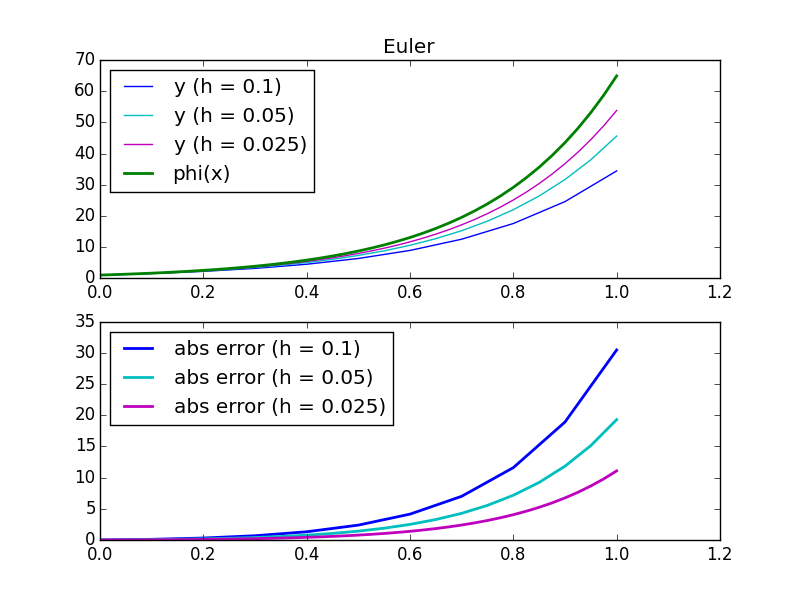
\includegraphics[width=1.0\textwidth]{plots/Euler.png}
\caption{\label{fig:euler}Gráfico mostrando o desempenho do método de Euler para cada valor de tamanho de passo $h$, bem como o erro absoluto associado para cada avaliação do método.}
\end{figure}

\begin{table}[!h]
\centering
\begin{tabular}{l*{6}{c}r}

x               & $h=0.1$ & $phi(x)$ \\
\hline
0                   & 1.0 & 1.0          \\
0.1                 & 1.5 & 1.60904183   \\
0.2                 & 2.19 & 2.50532985   \\
0.3                 & 3.146 & 3.83013885   \\
0.4                 & 4.4744 & 5.794226     \\
0.5                 & 6.32416 & 8.71200412   \\
0.6                 & 8.903824 & 13.05252195  \\
0.7                 & 12.5053536 & 19.51551804  \\
0.8                 & 17.53749504 & 29.14487961  \\
0.9                 & 24.57249306 & 43.4979034   \\
1.0                 & 34.41149028 & 64.89780316  \\
\end{tabular}
\caption{\label{tab:euler}Tabela comparativa para diferentes valores de $h$.}
\end{table}


\pagebreak 





\subsection{Euler Inverso}

O método de Euler Inverso é definido pela seguinte equação:

\begin{equation}
y_{n+1} = y_{n} + hf(x_{n+1},y_{n+1})
\end{equation}

Este método é classificado como método implícito por utilizar do lado direito de sua expressão o mesmo termo que se procura estimar, i.e. $y_{n+1}$.


Na figura \ref{fig:beuler} são mostrados diferentes aproximações geradas por diferentes valores de de $h$ para a solução exata da Eq (\ref{eq:problema}), $phi(x)$. Logo abaixo também é mostrado a evolução do erro absoluto para cada avaliação do método, dado o correspondente tamanho do passo $h$. Na tabela \ref{tab:beuler} apresenta do desempenho do método de Euler Inverso para diferentes tamanhos de passo $h$.



\begin{figure}[!h]
\centering
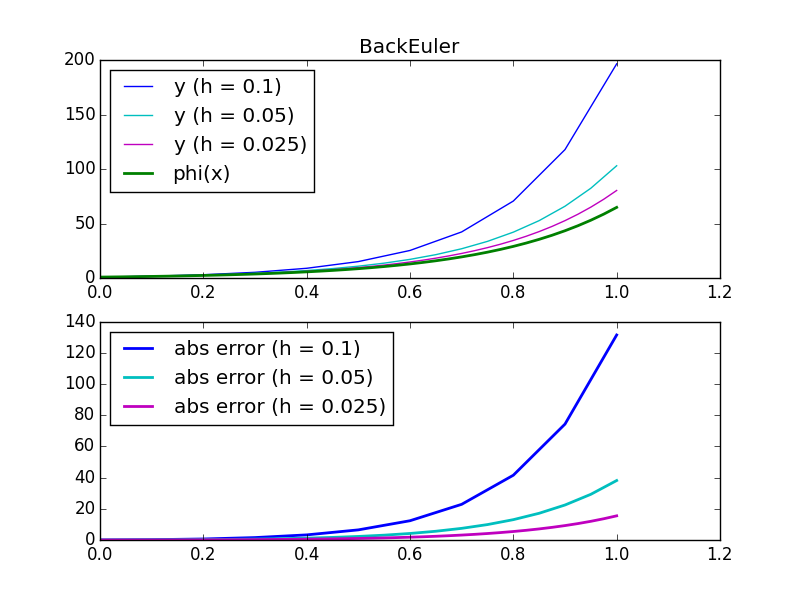
\includegraphics[width=1.0\textwidth]{plots/BackEuler.png}
\caption{\label{fig:beuler}Gráfico mostrando o desempenho do método de Euler Inverso para cada valor de tamanho de passo $h$, bem como o erro absoluto associado para cada avaliação do método.}
\end{figure}

\begin{table}[!h]
\centering
\begin{tabular}{l*{6}{c}r}

x               & $h=0.1$ & $phi(x)$ \\
\hline
0                   & 1.0 & 1.0          \\
0.1                 & 1.81666667 & 1.60904183   \\
0.2                 & 3.16111111 & 2.50532985   \\
0.3                 & 5.38518519 & 3.83013885   \\
0.4                 & 9.07530864 & 5.794226     \\
0.5                 & 15.20884774 & 8.71200412   \\
0.6                 & 25.41474623 & 13.05252195  \\
0.7                 & 42.40791038 & 19.51551804  \\
0.8                 & 70.71318397 & 29.14487961  \\
0.9                 & 117.87197328 & 43.4979034   \\
1.0                 & 196.45328879 & 64.89780316  \\
\end{tabular}
\caption{\label{tab:beuler}Tabela comparativa para diferentes valores de $h$.}
\end{table}

\pagebreak

\subsection{Euler Aprimorado}

O método de Euler Aprimorado é definido pela seguinte equação:

\begin{equation}
\label{eq:impeuler}
y_{n+1} = y_{n} + h\frac{(f(x_{n},y_{n})+f(x_{n+1},y_{n+1}))}{2}
\end{equation}

O Euler Aprimorado apresenta uma aproximação trapezoidal para o termo integral em \ref{eq:impeuler}.

Na figura \ref{fig:impeuler} são mostrados diferentes aproximações geradas por diferentes valores de de $h$ para a solução exata da Eq (\ref{eq:problema}), $phi(x)$. Logo abaixo também é mostrado a evolução do erro absoluto para cada avaliação do método, dado o correspondente tamanho do passo $h$. Na tabela \ref{tab:impeuler} apresenta do desempenho do método de Euler para diferentes tamanhos de passo $h$.

\begin{figure}[!h]
\centering
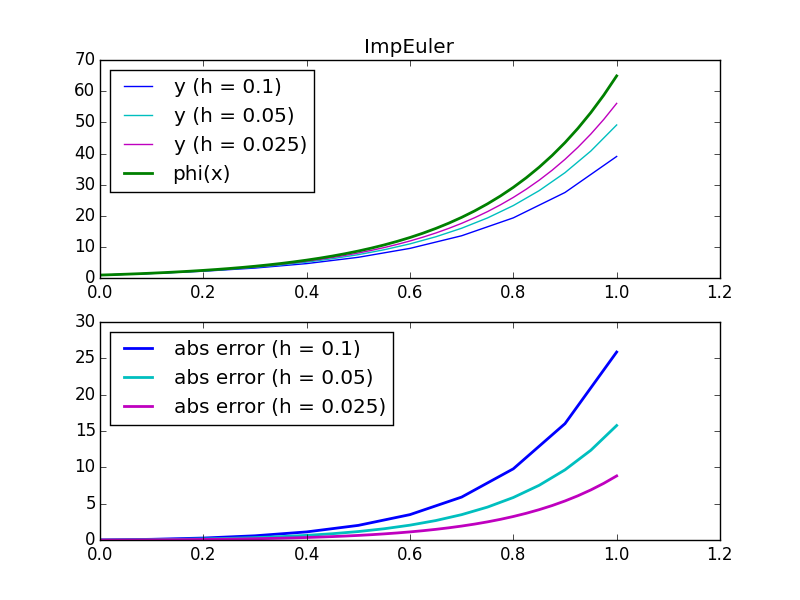
\includegraphics[width=1.0\textwidth]{plots/ImpEuler.png}
\caption{\label{fig:impeuler}Gráfico mostrando o desempenho do método de Euler Aprimorado para cada valor de tamanho de passo $h$, bem como o erro absoluto associado para cada avaliação do método.}
\end{figure}

\begin{table}[!h]
\centering
\begin{tabular}{l*{6}{c}r}
x               & $h=0.1$ & $phi(x)$ \\
\hline
0                   & 1.0 & 1.0          \\
0.1                 & 1.515 & 1.60904183   \\
0.2                 & 2.2363 & 2.50532985   \\
0.3                 & 3.250546 & 3.83013885   \\
0.4                 & 4.68077532 & 5.794226     \\
0.5                 & 6.70170095 & 8.71200412   \\
0.6                 & 9.56141536 & 13.05252195  \\
0.7                 & 13.6122098 & 19.51551804  \\
0.8                 & 19.35433792 & 29.14487961  \\
0.9                 & 27.49815985 & 43.4979034   \\
1.0                 & 39.05238699 & 64.89780316  \\
\end{tabular}
\caption{\label{tab:impeuler}Tabela comparativa para diferentes valores de $h$.}
\end{table}

\pagebreak

\subsection{Runge-Kutta}

O método de Runge-Kutta é definido pela seguinte equação:

\begin{equation}
\label{eq:rkutta}
y_{n+1} = y_n + \frac{h}{6}\left(k_1 + 2k_2 + 2k_3 + k_4 \right)
\end{equation}

Onde,

\begin{subequations}
\begin{align}
k_1 = f(t_n, y_n),
\\
k_2 = f(t_n + \tfrac{h}{2}, y_n + \tfrac{1}{2} k_1 h),
\\
k_3 = f(t_n + \tfrac{h}{2}, y_n + \tfrac{1}{2} k_2 h),
\\
k_4 = f(t_n + h, y_n + k_3 h).
\end{align}
\end{subequations}

Runge-Kutta apresenta uma aproximação bastante robusta, pois aproxima o termo integral utilizando uma média ponderada de várias aproximações intermediarias.

Na figura \ref{fig:rkutta} são mostrados diferentes aproximações geradas por diferentes valores de de $h$ para a solução exata da Eq (\ref{eq:problema}), $phi(x)$. Logo abaixo também é mostrado a evolução do erro absoluto para cada avaliação do método, dado o correspondente tamanho do passo $h$. Na tabela \ref{tab:rkutta} apresenta do desempenho do método de Euler para diferentes tamanhos de passo $h$.

\begin{figure}[!h]
\centering
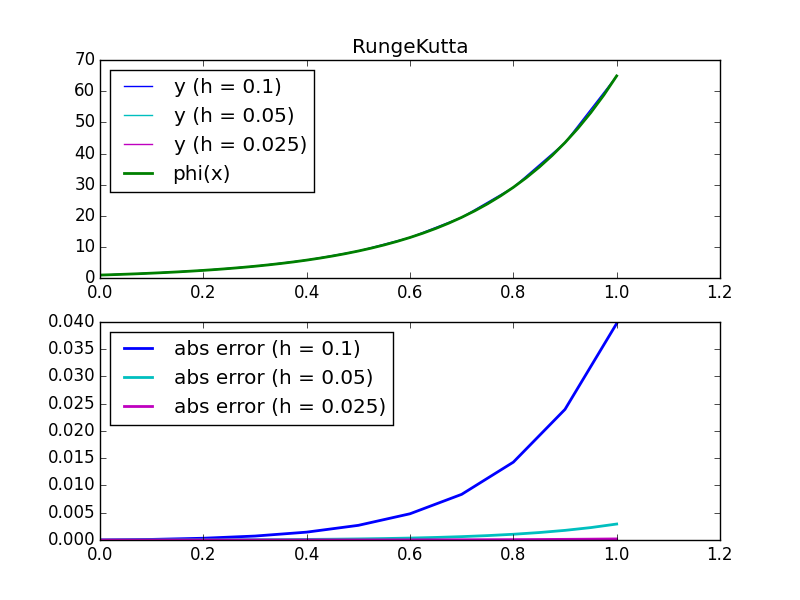
\includegraphics[width=1.0\textwidth]{plots/RungeKutta.png}
\caption{\label{fig:rkutta}Gráfico mostrando o desempenho do método de Runge-Kutta para cada valor de tamanho de passo $h$, bem como o erro absoluto associado para cada avaliação do método.}
\end{figure}

\begin{table}[!h]
\centering
\begin{tabular}{l*{6}{c}r}
x               & $h=0.1$ & $phi(x)$ \\
\hline
0                   & 1.0 & 1.0          \\
0.1                 & 1.60893333 & 1.60904183   \\
0.2                 & 2.50500615 & 2.50532985   \\
0.3                 & 3.82941451 & 3.83013885   \\
0.4                 & 5.79278527 & 5.794226     \\
0.5                 & 8.70931755 & 8.71200412   \\
0.6                 & 13.04771263 & 13.05252195  \\
0.7                 & 19.50714785 & 19.51551804  \\
0.8                 & 29.13060936 & 29.14487961  \\
0.9                 & 43.47395433 & 43.4979034   \\
1.0                 & 64.85810681 & 64.89780316  \\
\end{tabular}
\caption{\label{tab:rkutta}Tabela comparativa para diferentes valores de $h$.}
\end{table}

\pagebreak



\subsection{Série de Taylor de Três Termos}

O método da Série de Taylor de Três Termos é definido pela seguinte equação:

\begin{equation}
\label{eq:taylor}
y_{n+1} = y_{n} + hy'_{n} + \frac{h^2}{2}y''_{n}
\end{equation}

Onde,

\begin{subequations}
\begin{align}
y'_{n} = f(t_n, y_n),
\\
y''_{n} = \tfrac{{\partial f(t_n, y_n)}}{{\partial x}} + \tfrac{{\partial f(t_n, y_n)}}{{\partial y}}y'_{n}.
\end{align}
\end{subequations}

Na figura \ref{fig:taylor} são mostrados diferentes aproximações geradas por diferentes valores de de $h$ para a solução exata da Eq (\ref{eq:problema}), $phi(x)$. Logo abaixo também é mostrado a evolução do erro absoluto para cada avaliação do método, dado o correspondente tamanho do passo $h$. Na tabela \ref{tab:taylor} apresenta do desempenho do método de Euler para diferentes tamanhos de passo $h$.

\begin{figure}[!h]
\centering
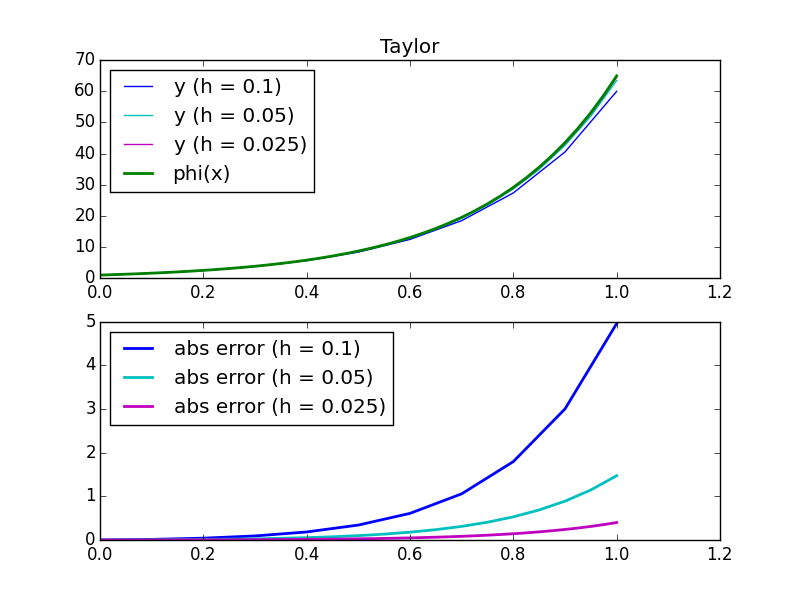
\includegraphics[width=1.0\textwidth]{plots/Taylor.png}
\caption{\label{fig:taylor}Gráfico mostrando o desempenho do método da Série de Taylor de Três Termos para cada valor de tamanho de passo $h$, bem como o erro absoluto associado para cada avaliação do método.}
\end{figure}

\begin{table}[!h]
\centering
\begin{tabular}{l*{6}{c}r}
x               & $h=0.1$ & $phi(x)$ \\
\hline
0                   & 1.0 & 1.0          \\
0.1                 & 1.595 & 1.60904183   \\
0.2                 & 2.4636 & 2.50532985   \\
0.3                 & 3.737128 & 3.83013885   \\
0.4                 & 5.60994944 & 5.794226     \\
0.5                 & 8.36972517 & 8.71200412   \\
0.6                 & 12.44219325 & 13.05252195  \\
0.7                 & 18.45744601 & 19.51551804  \\
0.8                 & 27.3480201 & 29.14487961  \\
0.9                 & 40.49406975 & 43.4979034   \\
1.0                 & 59.93822323 & 64.89780316  \\
\end{tabular}
\caption{\label{tab:taylor}Tabela comparativa para diferentes valores de $h$.}
\end{table}

\pagebreak

\section{Métodos de Passo Múltiplo}

Métodos de Passo Múltiplo se diferem dos métodos anteriores no sentido de utilizarem informação associada a vários pontos do passado ($y_{n}, y_{n-1},..., y_{n-k}$) na estimativa do próximo $y_{n+1}$. Essa abordagem, portanto, contrasta diretamente com os métodos númericos vistos na seção anterior, o quais se utilizam apenas do valor computado imediamente anterior para estimar $y_{n+1}$. 

\subsection{Adams-Bashforth}

Os métodos de Adams-Bashforth representam uma família de métodos numéricos explicitos para solução do problema de valor inicial pra equações diferenciais lineares de primeira ordem. O princípio fundamental dessa família de métodos se baseia na aproximação da função $y'_{n} = f(x_n,y_n)$ por meio de um polinônomio arbitrário $P_k(x)$ de grau $k$. O grau desse polinômio escolhido representa a ordem do método de Adams-Bashforth. As equações para cada ordem do método deste método são obtidas ao se fazer interpolação exata por $k+1$ pontos, $(x_n,y_n),(x_{n-1},y_{n-1}),...,(x_{n-k},y_{n-k})$, dessa forma são determinados os coeficientes do polinômio de grau grau $k$ que interpola esses pontos $P_k(x)$. Como esse polinômio representa $f(x_n,y_n) = P_k(x)$, a expressão final dos métodos de Adams-Bashforth de ordem $k$ é dada pela equação abaixo.

\begin{equation}
\label{eq:bashforth}
y_{n+1} = y_{n} + \int_{x_{n}}^{x_{n+1}} \mathrm{P_k(x)}\,\mathrm{d}x
\end{equation}
\\
Neste projeto foram implementados os métodos de ordem 1, 2, 3 e 4 representados pelas respectivas equações abaixo.
\vspace{10mm} %5mm vertical space
\\
$1^a$ Ordem: 

\begin{equation}
\label{eq:bashforth1}
y_{n+2} = y_{n+1} + h\left( \frac{3}{2}f(t_{n+1}, y_{n+1}) - \frac{1}{2}f(t_n, y_n) \right)
\end{equation}
\\
$2^a$ Ordem: 

\begin{equation}
\label{eq:bashforth2}
y_{n+3} = y_{n+2} + h\left( \frac{23}{12} f(t_{n+2}, y_{n+2}) - \frac43 f(t_{n+1}, y_{n+1}) + \frac{5}{12}f(t_n, y_n)\right)
\end{equation}
\\
$3^a$ Ordem: 

\begin{equation}
\label{eq:bashforth3}
y_{n+4} = y_{n+3} + h\left( \frac{55}{24} f(t_{n+3}, y_{n+3}) - \frac{59}{24} f(t_{n+2}, y_{n+2}) +  \frac{37}{24} f(t_{n+1}, y_{n+1}) - \frac{3}{8} f(t_n, y_n) \right)
\end{equation}
\\
$4^a$ Ordem: 

\begin{dmath}
\label{eq:bashforth4}
y_{n+5} = y_{n+4} + h\left( \frac{1901}{720} f(t_{n+4}, y_{n+4}) - \frac{1387}{360} f(t_{n+3}, y_{n+3}) + \frac{109}{30} f(t_{n+2}, y_{n+2}) - \frac{637}{360} f(t_{n+1}, y_{n+1}) + \frac{251}{720} f(t_n, y_n) \right)
\end{dmath}
\begin{figure}[!htb]
\centering
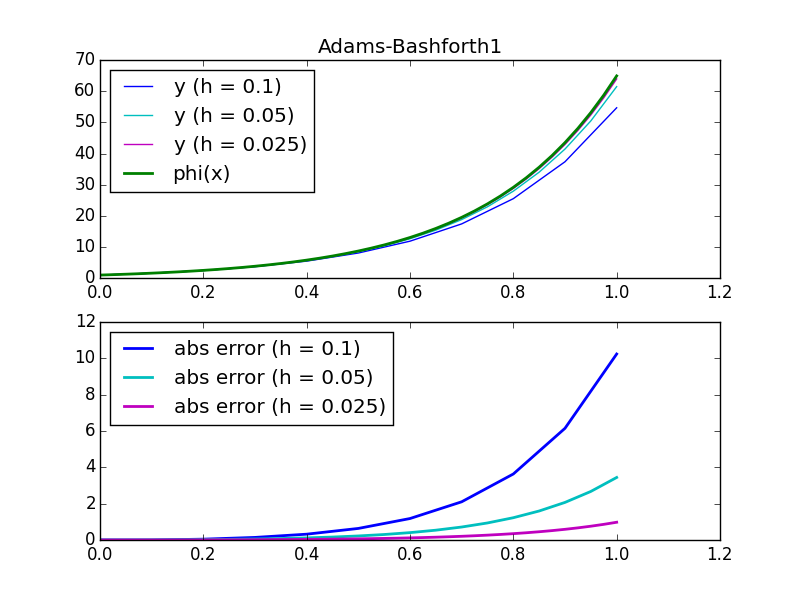
\includegraphics[width=1.0\textwidth]{plots/Adams-Bashforth1.png}
\caption{\label{fig:bashforth1}Gráfico Adams-Bashforth ($1^a$ Ordem) para valores de h iguais a 0.1, 0.05, 0.025.}
\end{figure}

\begin{table}[!h]
\centering

\begin{tabular}{l*{6}{c}r}
x               & $h=0.1$ & $phi(x)$ \\
\hline
0                   & 1.0 & 1.0          \\
0.1                 & 1.60893333 & 1.60904183   \\
0.2                 & 2.45929333 & 2.50532985   \\
0.3                 & 3.68808267 & 3.83013885   \\
0.4                 & 5.4740736 & 5.794226     \\
0.5                 & 8.07590123 & 8.71200412   \\
0.6                 & 11.87162724 & 13.05252195  \\
0.7                 & 17.41442334 & 19.51551804  \\
0.8                 & 25.5137519 & 29.14487961  \\
0.9                 & 37.35411837 & 43.4979034   \\
1.0                 & 54.66883901 & 64.89780316  \\
\end{tabular}
\caption{\label{tab:bashforth1}Tabela comparativa Adams-Bashforth ($1^a$ Ordem) e solução exata ($h=0.1$).}
\end{table}
%%%%%%%%%%%% COMMENT 

\begin{figure}[b]
\centering
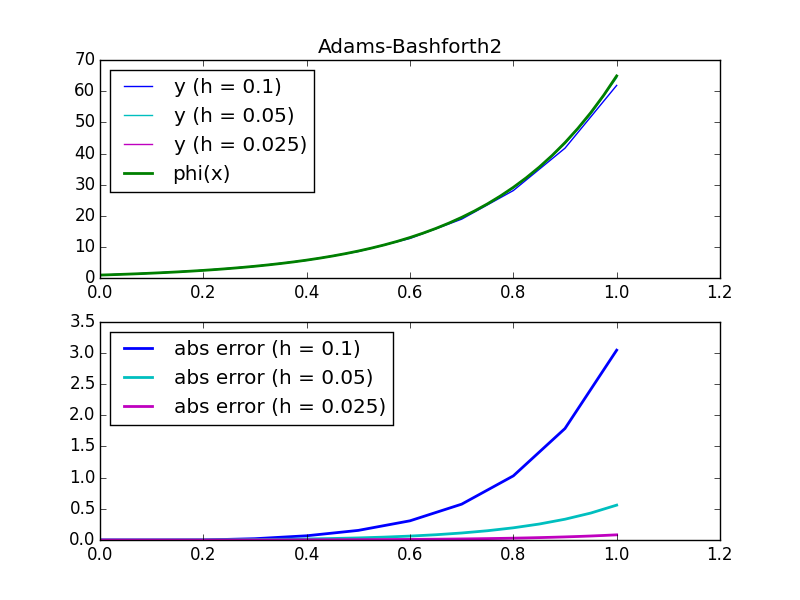
\includegraphics[width=1.0\textwidth]{plots/Adams-Bashforth2.png}
\caption{\label{fig:bashforth2}Gráfico Adams-Bashforth ($2^a$ Ordem) para valores de h iguais a 0.1, 0.05, 0.025.}
\end{figure}


\begin{figure}[b]
\centering
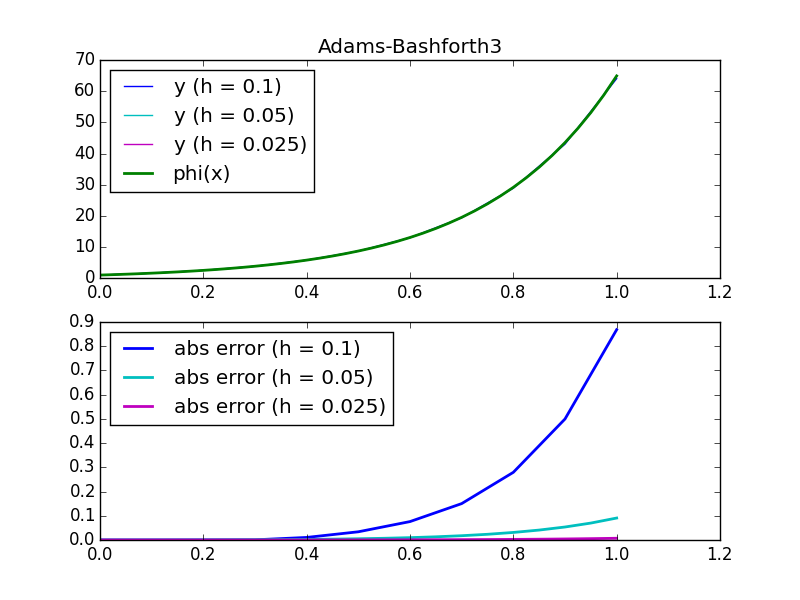
\includegraphics[width=1.0\textwidth]{plots/Adams-Bashforth3.png}
\caption{\label{fig:bashforth3}Gráfico Adams-Bashforth ($3^a$ Ordem) para valores de h iguais a 0.1, 0.05, 0.025.}
\end{figure}



\begin{figure}[b]
\centering
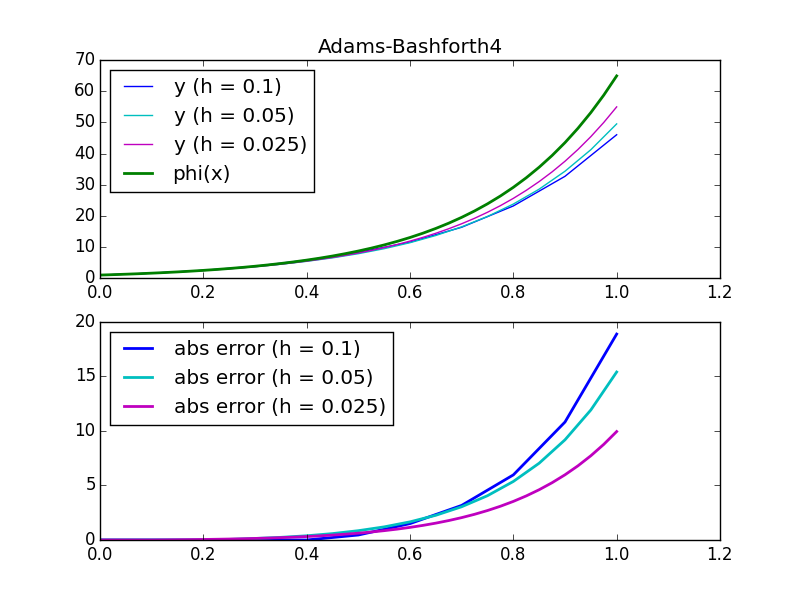
\includegraphics[width=1.0\textwidth]{plots/Adams-Bashforth4.png}
\caption{\label{fig:bashforth4}Gráfico Adams-Bashforth ($4^a$ Ordem) para valores de h iguais a 0.1, 0.05, 0.025.}
\end{figure}

\pagebreak
\subsection{Adams-Multon}

O método de Adams-Multon segue um princípio bastante similar ao do Adams-Bashforth. A diferença é que sua expressão é encontrada ao se definir uma interpolação polinomial de grau $k$ passando pelos pontos $(x_n,y_n),(x_{n-1},y_{n-1}),...,(x_{n-(k-1)},y_{n-(k-1)})$ e $(x_{n+1},y_{n+1})$, isso implica que este é também um método implicito.

Nesse projeto foram implementados os métodos de ordem 1, 2, 3 e 4 representados pelas respectivas equações abaixo.
\vspace{5mm} %5mm vertical space

$1^a$ Ordem: 

\begin{dmath}
\label{eq:multon1}
y_{n+1} = y_n + \frac{1}{2} h \left( f(t_{n+1},y_{n+1}) + f(t_n,y_n) \right) \\
\end{dmath}

$2^a$ Ordem: 
\begin{dmath}
\label{eq:multon2}
y_{n+2} = y_{n+1} + h \left( \frac{5}{12} f(t_{n+2},y_{n+2}) + \frac{2}{3} f(t_{n+1},y_{n+1}) - \frac{1}{12} f(t_n,y_n) \right)
\end{dmath}

$3^a$ Ordem: 

\begin{dmath}
\label{eq:multon3}
y_{n+3} = y_{n+2} + h \left( \frac{3}{8} f(t_{n+3},y_{n+3}) + \frac{19}{24} f(t_{n+2},y_{n+2}) - \frac{5}{24} f(t_{n+1},y_{n+1}) + \frac{1}{24} f(t_n,y_n) \right) \\
\end{dmath}

$4^a$ Ordem: 

\begin{dmath}
\label{eq:multon4}
y_{n+4} = y_{n+3} + h \left( \frac{251}{720} f(t_{n+4},y_{n+4}) + \frac{646}{720} f(t_{n+3},y_{n+3}) - \frac{264}{720} f(t_{n+2},y_{n+2}) + \frac{106}{720} f(t_{n+1},y_{n+1}) - \frac{19}{720} f(t_n,y_n) \right)
\end{dmath}

\begin{figure}[!htb]
\centering
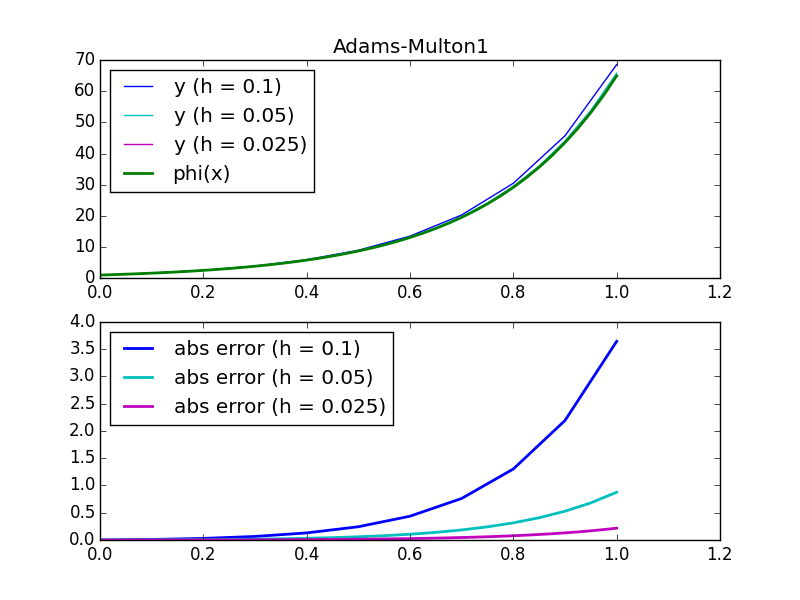
\includegraphics[width=1.0\textwidth]{plots/Adams-Multon1.png}
\caption{\label{fig:multon1}Gráfico Adams-Bashforth ($1^a$ Ordem) para valores de h iguais a 0.1, 0.05, 0.025.}
\end{figure}

\begin{table}[!h]
\centering
\begin{tabular}{l*{6}{c}r}
x               & $h=0.1$ & $phi(x)$ \\
\hline
0                   & 1.0 & 1.0          \\
0.1                 & 1.61875 & 1.60904183   \\
0.2                 & 2.534375 & 2.50532985   \\
0.3                 & 3.8953125 & 3.83013885   \\
0.4                 & 5.92421875 & 5.794226     \\
0.5                 & 8.95507812 & 8.71200412   \\
0.6                 & 13.48886719 & 13.05252195  \\
0.7                 & 20.27705078 & 19.51551804  \\
0.8                 & 30.44682617 & 29.14487961  \\
0.9                 & 45.68898926 & 43.4979034   \\
1.0                 & 68.53973389 & 64.89780316  \\
\end{tabular}
\caption{\label{tab:multon1}Tabela comparativa Adams-Multon ($1^a$ Ordem) e solução exata ($h=0.1$).}
\end{table}

\begin{figure}[b]
\centering
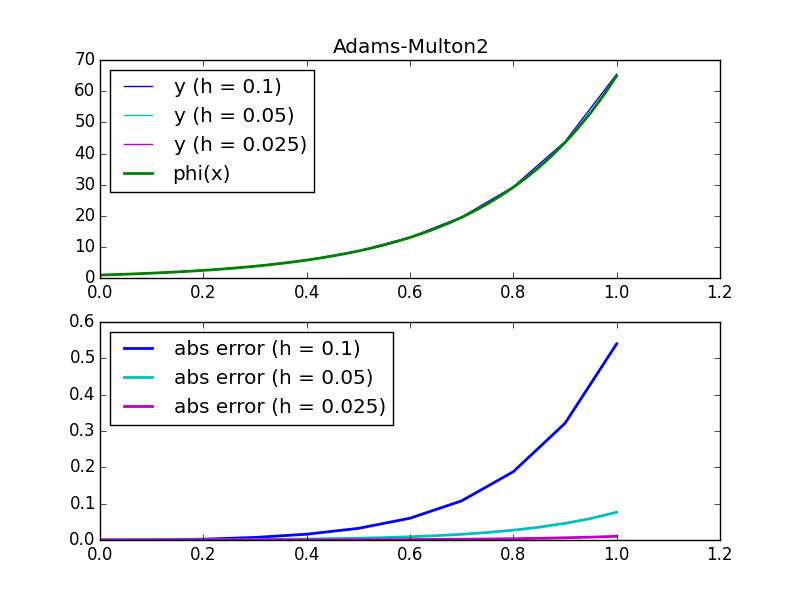
\includegraphics[width=1.0\textwidth]{plots/Adams-Multon2.png}
\caption{\label{fig:multon2}Gráfico Adams-Multon ($2^a$ Ordem) para valores de h iguais a 0.1, 0.05, 0.025.}
\end{figure}


\begin{figure}[b]
\centering
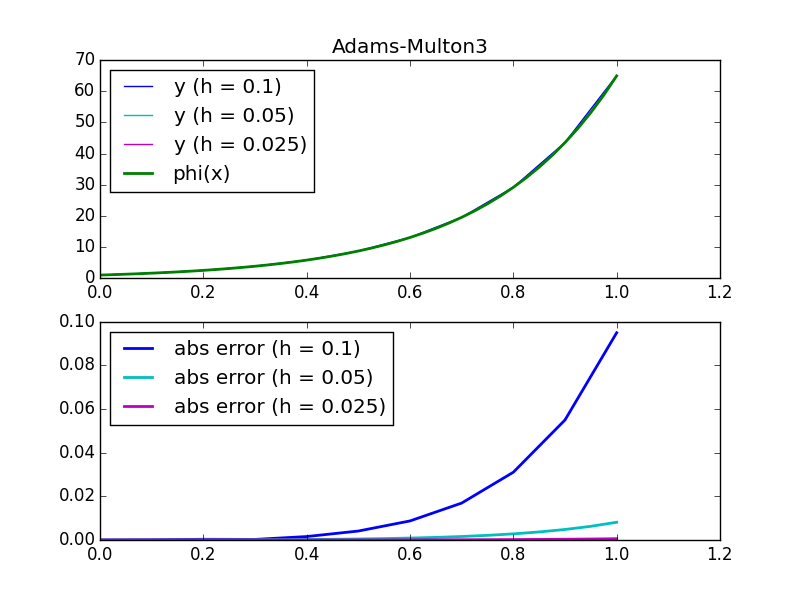
\includegraphics[width=1.0\textwidth]{plots/Adams-Multon3.png}
\caption{\label{fig:multon3}Gráfico Adams-Multon ($3^a$ Ordem) para valores de h iguais a 0.1, 0.05, 0.025.}
\end{figure}



\begin{figure}[b]
\centering
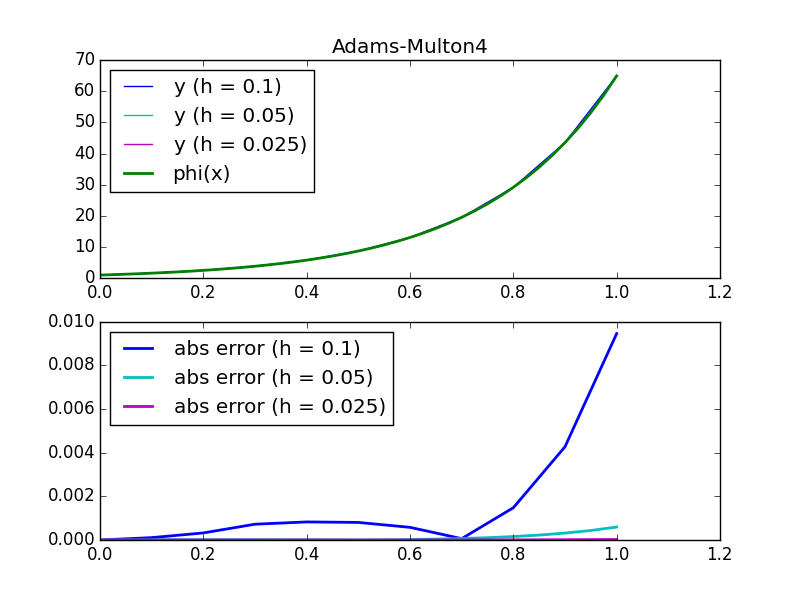
\includegraphics[width=1.0\textwidth]{plots/Adams-Multon4.png}
\caption{\label{fig:multon4}Gráfico Adams-Multon ($4^a$ Ordem) para valores de h iguais a 0.1, 0.05, 0.025.}
\end{figure}

\pagebreak

\subsection{Predição e Correção}

Métodos que utilizam predição e correção removem a implicidade de métodos como o Adams-Multon ao utilizar métodos explicitos como o Adams-Bashforth como preditores. Usando esta predição, gera-se uma estimativa corrigida a partir desse resultado, ao invés de se estimar o ponto $y_{n+1}$ implicitamente. Esse ciclo pode ser repetido iterativamente até que correção feita pelo Adams-Multon não seja mais significativa (menor que um limiar). Esse tipo de método fornece a possibilidade de definição de vários variantes adaptativos, i.e. métodos que ajustam o tamanho do passo $h=1$ em tempo de execução de acordo com o comportamento do erro de ajuste.
\\
Neste projeto foram implementados os métodos de predição e correção de ordem 1, 2, 3 e 4 utilizando-se o Adams-Bashforth como preditor, e Adams-Multon de correspondente ordem como corretor. As equações para tais métodos são:
\vspace{10mm} %5mm vertical space
\\
$1^a$ Ordem: 

\begin{dmath}
\label{eq:pc1}
y_{n+1} = y_n + \frac{1}{2} h \left( f(t_{n+1},\gamma_{n+1}) + f(t_n,y_n) \right) \\
\end{dmath}
Onde $\gamma_{n+1}$ é dado pela Eq (\ref{eq:bashforth1}), ou seja esta é a estimativa a ser corrigida pelo adams-multon.
\\
$2^a$ Ordem: 
\begin{dmath}
\label{eq:pc2}
y_{n+2} = y_{n+1} + h \left( \frac{5}{12} f(t_{n+2},\gamma_{n+2}) + \frac{2}{3} f(t_{n+1},y_{n+1}) - \frac{1}{12} f(t_n,y_n) \right)
\end{dmath}
Onde $\gamma_{n+2}$ é dado pela Eq (\ref{eq:bashforth2}), ou seja esta é a estimativa a ser corrigida pelo adams-multon.

$3^a$ Ordem: 

\begin{dmath}
\label{eq:pc3}
y_{n+3} = y_{n+2} + h \left( \frac{3}{8} f(t_{n+3},\gamma_{n+3}) + \frac{19}{24} f(t_{n+2},y_{n+2}) - \frac{5}{24} f(t_{n+1},y_{n+1}) + \frac{1}{24} f(t_n,y_n) \right) \\
\end{dmath}
Onde $\gamma_{n+3}$ é dado pela Eq (\ref{eq:bashforth3}), ou seja esta é a estimativa a ser corrigida pelo adams-multon.

$4^a$ Ordem: 

\begin{dmath}
\label{eq:pc4}
y_{n+4} = y_{n+3} + h \left( \frac{251}{720} f(t_{n+4},\gamma_{n+4}) + \frac{646}{720} f(t_{n+3},y_{n+3}) - \frac{264}{720} f(t_{n+2},y_{n+2}) + \frac{106}{720} f(t_{n+1},y_{n+1}) - \frac{19}{720} f(t_n,y_n) \right)
\end{dmath}
Onde $\gamma_{n+4}$ é dado pela Eq (\ref{eq:bashforth4}), ou seja esta é a estimativa a ser corrigida pelo adams-multon.

\begin{figure}[!htb]
\centering
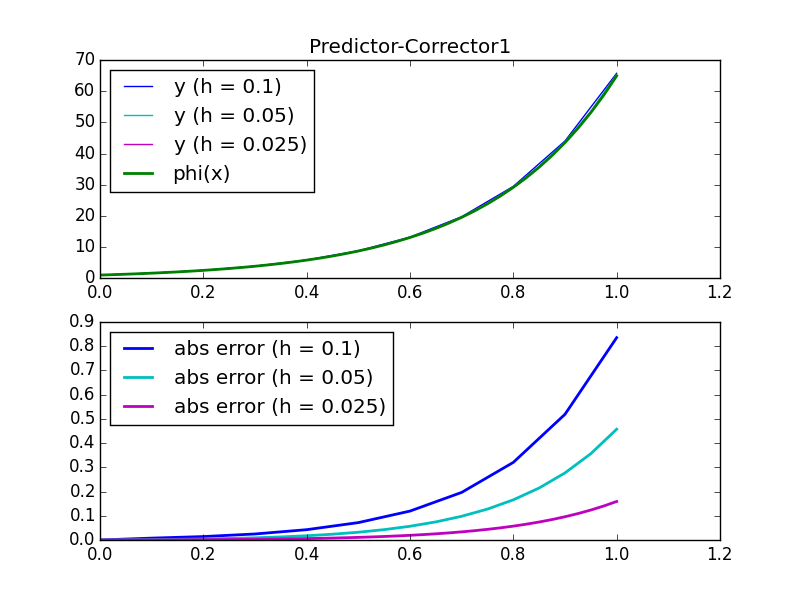
\includegraphics[width=1.0\textwidth]{plots/Predictor-Corrector1.png}
\caption{\label{fig:pc1}Gráfico Predição e Correção ($1^a$ Ordem) para valores de h iguais a 0.1, 0.05, 0.025.}
\end{figure}

\begin{table}[!h]
\centering
\begin{tabular}{l*{6}{c}r}
x               & $h=0.1$ & $phi(x)$ \\
\hline
0                   & 1.0 & 1.0          \\
0.1                 & 1.61678667 & 1.60904183   \\
0.2                 & 2.51951573 & 2.50532985   \\
0.3                 & 3.85499245 & 3.83013885   \\
0.4                 & 5.83680789 & 5.794226     \\
0.5                 & 8.7837483 & 8.71200412   \\
0.6                 & 13.1718251 & 13.05252195  \\
0.7                 & 19.71182421 & 19.51551804  \\
0.8                 & 29.4650998 & 29.14487961  \\
0.9                 & 44.01647873 & 43.4979034   \\
1.0                 & 65.73244368 & 64.89780316  \\
\end{tabular}
\caption{\label{tab:pc1}Tabela comparativa Predição e Correção ($1^a$ Ordem) e solução exata ($h=0.1$).}
\end{table}

\begin{figure}[b]
\centering
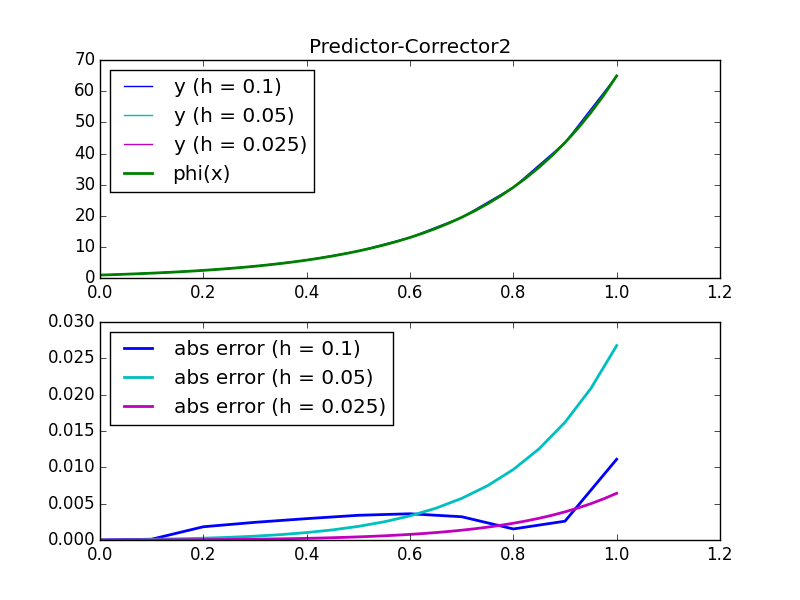
\includegraphics[width=1.0\textwidth]{plots/Predictor-Corrector2.png}
\caption{\label{fig:pc1}Gráfico Predição e Correção ($2^a$ Ordem) para valores de h iguais a 0.1, 0.05, 0.025.}
\end{figure}

\begin{figure}[b]
\centering
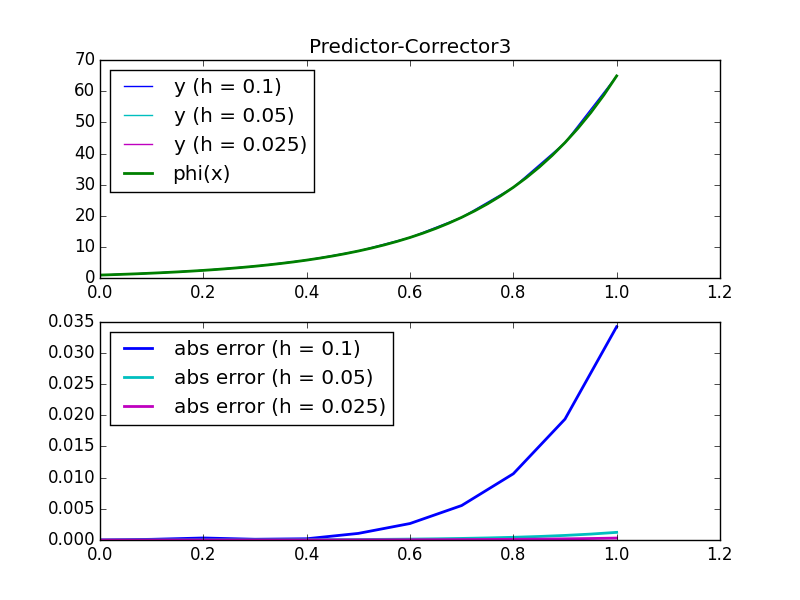
\includegraphics[width=1.0\textwidth]{plots/Predictor-Corrector3.png}
\caption{\label{fig:pc2}Gráfico Predição e Correção ($3^a$ Ordem) para valores de h iguais a 0.1, 0.05, 0.025.}
\end{figure}
\begin{figure}[b]
\centering
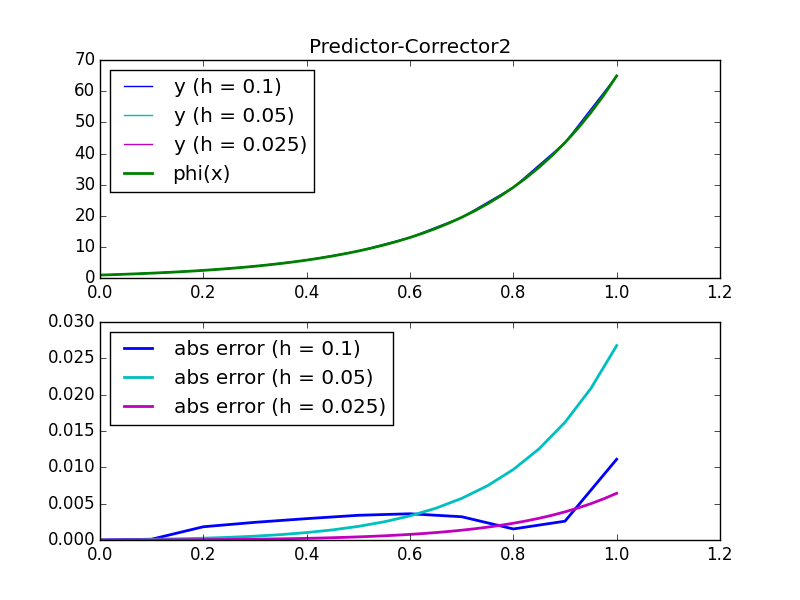
\includegraphics[width=1.0\textwidth]{plots/Predictor-Corrector2.png}
\caption{\label{fig:pc3}Gráfico Predição e Correção ($4^a$ Ordem) para valores de h iguais a 0.1, 0.05, 0.025.}
\end{figure}

\subsection{Diferenciação Inversa}

Foram implementados os métodos de diferenciação inversa de ordem 1, 2, 3 e 4. Para cada ordem, os métodos de diferencição inversa são dados pelas equações abaixo.
\vspace{10mm} %5mm vertical space
\\
\\*
$1^a$ Ordem: 

\begin{dmath}
\label{eq:backdiff1}
y_{n+1} = y_n + h f(t_{n+1}, y_{n+1}) \\
\end{dmath}

$2^a$ Ordem: 
\begin{dmath}
\label{eq:backdiff2}
y_{n+2} = \tfrac43 y_{n+1} - \tfrac13 y_n + \tfrac23 h f(t_{n+2}, y_{n+2});
\end{dmath}

$3^a$ Ordem: 

\begin{dmath}
\label{eq:backdiff3}
y_{n+3}  = \tfrac{18}{11} y_{n+2} - \tfrac9{11} y_{n+1} + \tfrac2{11} y_n + \tfrac6{11} h f(t_{n+3}, y_{n+3})
\end{dmath}

$4^a$ Ordem: 

\begin{dmath}
\label{eq:backdiff4}
y_{n+4} = \tfrac{48}{25} y_{n+3} - \tfrac{36}{25} y_{n+2} + \tfrac{16}{25} y_{n+1} - \tfrac{3}{25} y_n + \tfrac{12}{25} h f(t_{n+4}, y_{n+4}) 
\end{dmath}

\begin{figure}[!htb]
\centering
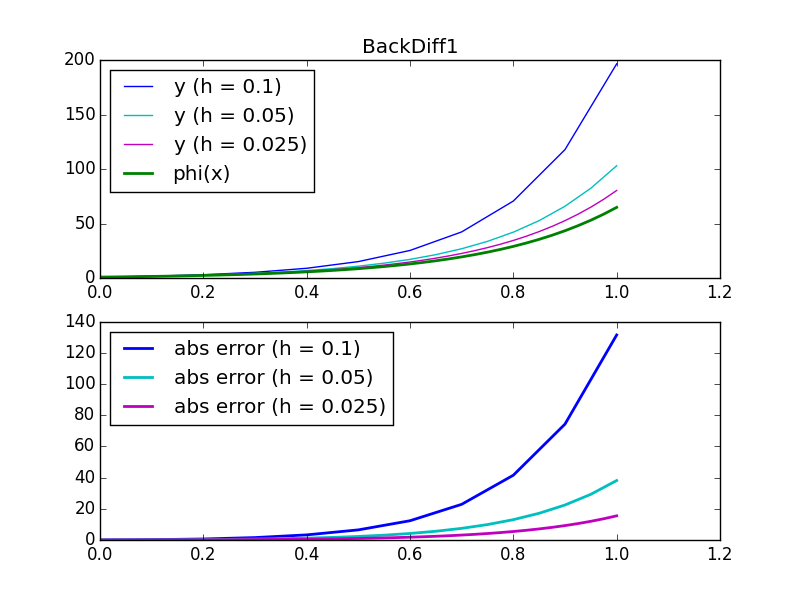
\includegraphics[width=1.0\textwidth]{plots/BackDiff1.png}
\caption{\label{fig:backdiff1}Gráfico Diferenciação Inversa ($1^a$ Ordem) para valores de h iguais a 0.1, 0.05, 0.025.}
\end{figure}

\begin{table}[!h]
\centering
\begin{tabular}{l*{6}{c}r}
x               & $h=0.1$ & $phi(x)$ \\
\hline
0                   & 1.0 & 1.0          \\
0.1                 & 1.81666667 & 1.60904183   \\
0.2                 & 3.16111111 & 2.50532985   \\
0.3                 & 5.38518519 & 3.83013885   \\
0.4                 & 9.07530864 & 5.794226     \\
0.5                 & 15.20884774 & 8.71200412   \\
0.6                 & 25.41474623 & 13.05252195  \\
0.7                 & 42.40791038 & 19.51551804  \\
0.8                 & 70.71318397 & 29.14487961  \\
0.9                 & 117.87197328 & 43.4979034   \\
1.0                 & 196.45328879 & 64.89780316  \\
\end{tabular}
\caption{\label{tab:backdiff1}Tabela comparativa Diferenciação Inversa ($1^a$ Ordem) e solução exata ($h=0.1$).}
\end{table}

\begin{figure}[b]
\centering
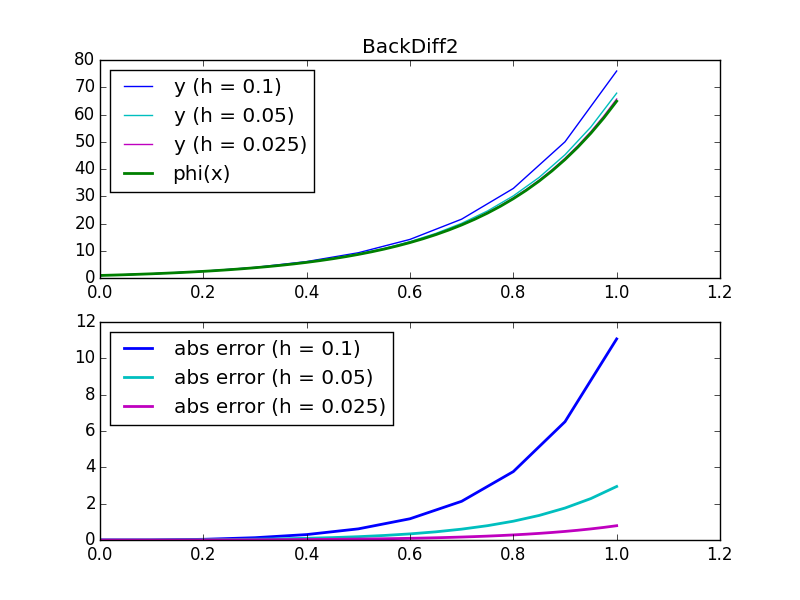
\includegraphics[width=1.0\textwidth]{plots/BackDiff2.png}
\caption{\label{fig:backdiff2}Gráfico Diferenciação Inversa ($2^a$ Ordem) para valores de h iguais a 0.1, 0.05, 0.025.}
\end{figure}

\begin{figure}[b]
\centering
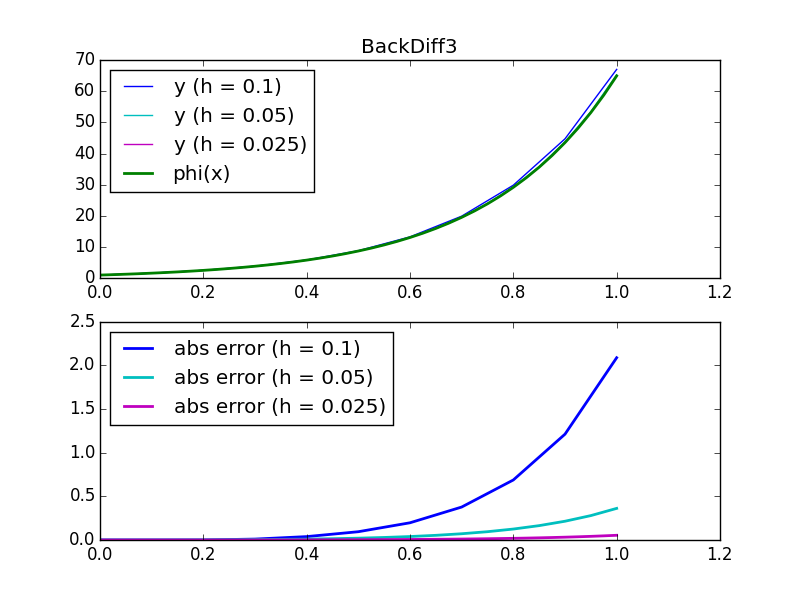
\includegraphics[width=1.0\textwidth]{plots/BackDiff3.png}
\caption{\label{fig:backdiff3}Gráfico Diferenciação Inversa ($3^a$ Ordem) para valores de h iguais a 0.1, 0.05, 0.025.}
\end{figure}

\begin{figure}[b]
\centering
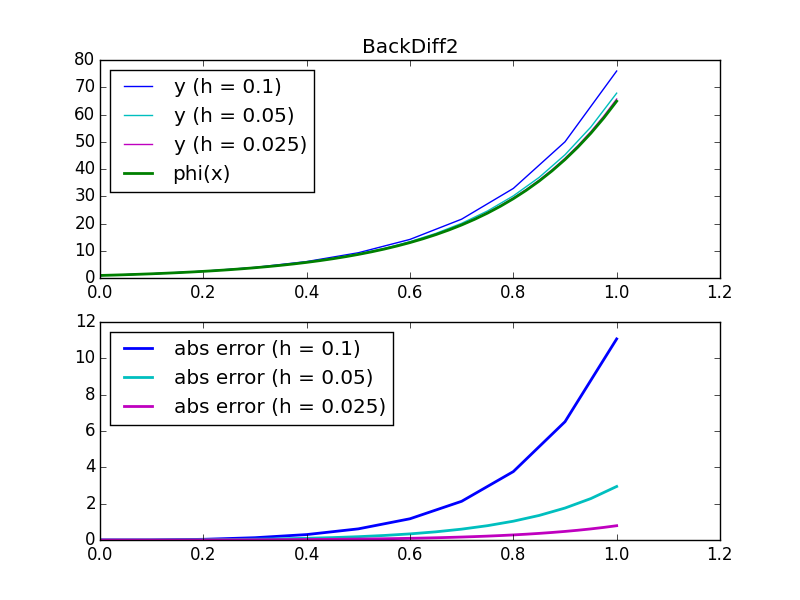
\includegraphics[width=1.0\textwidth]{plots/BackDiff2.png}
\caption{\label{fig:backdiff4}Gráfico Diferenciação Inversa ($4^a$ Ordem) para valores de h iguais a 0.1, 0.05, 0.025.}
\end{figure}

\pagebreak

\section{Conclusão}


Neste projeto foram implementados ao todo 21 métodos, sendo 5 métodos de Passo Único e 16 métodos de Passo Múltiplo. Os resultados dos métodos para o mesmo problema de valor inicial foram coletados brevemente comparados. Os resultados dizem respeito ao comportamento esperado para os métodos, com respectivos erros teóricos previstos. Neste projeto a análise dos métodos foi feita com base em uma solução analítica dada, no entando a importância desses métodos se dá ao ponto que para vários problemas do mundo real não possuem solução analítica, ou é simplismente inviável obtê-la. Foi visto também que alguns métodos apresentaram um desempenho melhor que outros, como foi o caso do Runge-Kutta, Série de Taylor de Três Termos, Adams, Previsão e Correção. A escolha do tamanho do passo $h$ também se mostra bastante importante como um meio de ajustar a qualidade da aproximação obtida, mesmo que com métodos inicialmente de pobre desempenho como o de Euler.

\section{Apêndice de Gráficos}


\end{document}